\chapter{Appendix}

\section{Known bugs and issues}

This section will list all known bugs and issues encountered during the development of the firmware.


\section{Fixed bugs and issues}

\subsection{Switching the \texttt{DE} pin seems inaccurate on higher speeds on the Raspberry Pi Zero2}
\label{subsec:de-bug}

This issue has been discovered on the Raspberry Pi Zero 2 which is used on the Test Setup V1.1 and has to do with toggling the \texttt{DE} pin of the RS-485 transceiver when the RPI wants to send data to the bus.
Serial uses a calculation to determine how long it should wait until the \texttt{DE} pin can be toggled from writing (1) back to reading (0) which is shown below in Listing \ref{lst:serial_write_delay}.

\begin{lstlisting}[frame=single, caption={Dynamic calculated sleep depending on length of data and baudrate}, captionpos=b, label={lst:serial_write_delay}, basicstyle=\small, style=CStyle]
     int time_to_sleep = (((float) length) / (float) ((float) baud / 10.0)) * 1000000.0;
\end{lstlisting}

The baudrate is the amount of bits that are send. Since we send 10 bits per byte (8 data bits, a start bit and a stop bit) we divide the baudrate by 10 to get the amount of bytes per second.
The total length of the data divided by the bytes per second leaves a delay expressed in seconds. Since we want some level of accuracy, we multiply it by a million and use the \texttt{usleep()} function.
When we test this formula on a baudrate of 9600 we can see that the \texttt{DE} pin is toggled right after the last bit is send. This can be seen in Figure \ref{fig:scope_no_extra_delay}.


\begin{figure}[H]
    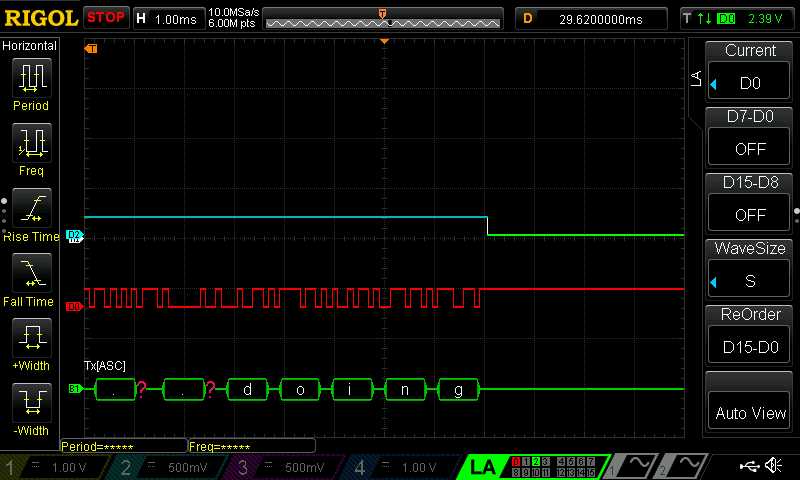
\includegraphics[scale=0.4]{figures/Scope_No_Extra_Delay.png}
    \caption{Baudrate 9600 and using the formula in Listing \ref{lst:serial_write_delay}, everything seems fine. \texttt{D2} is RS485 DE pin and \texttt{D0} is the TX pin}
    \label{fig:scope_no_extra_delay}
\end{figure}


\newpage
Because the Operating System on the RPI where this software is tested on, it might be safe to add a bit of extra timing in order to make sure that the data is on the bus. For instance, we could add 1 to \texttt{length} in Listing \ref{lst:serial_write_delay} to wait for an extra byte delay.
When we do so and send again on 9600 baud, we should expect a little above ~1.04 milliseconds extra delay before the \texttt{DE} pin is toggled.
This can be seen in Figure \ref{fig:scope_extra_delay9600} where the division is set to 1 millisecond. Indeed, the \texttt{DE} pin is toggled a little after ~1.04 milliseconds.

\begin{figure}[H]
    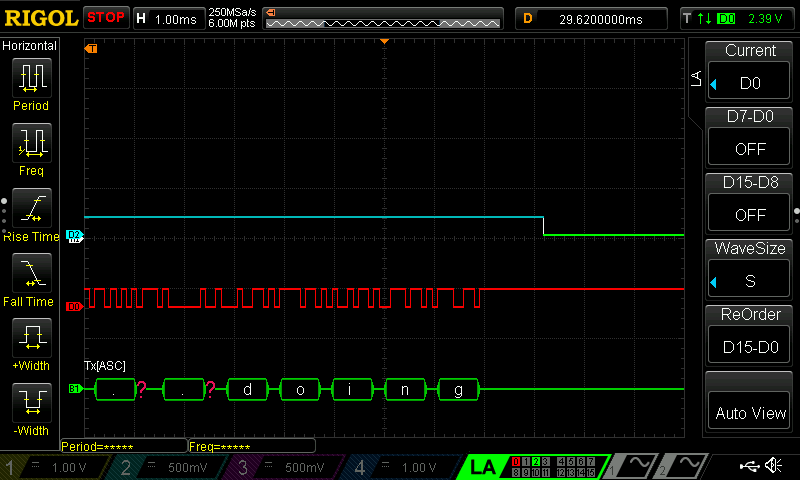
\includegraphics[scale=0.4]{figures/Scope_Extra_Delay9600.png}
    \caption{Baudrate 9600 and using the formula in Listing \ref{lst:serial_write_delay} but added 1 to \texttt{length}}
    \label{fig:scope_extra_delay9600}
\end{figure}

However, things start to get wacky on higher baudrates such as 115200.
In the example in Figure \ref{fig:scope_no_delay115200} we are sending 30 bytes.
This means we will sleep for $\frac{30}{11520} * 1000000 = 2604  \mu S$.
We can see that the \texttt{DE} pin stays up for \texttildelow3100 $\mu S$ without adding any extra delay in the formula in Listing \ref{lst:serial_write_delay} while the data seems to be okay but a bit on the higher end of the time spectrum.
The reason for this extra time could be that the \texttt{usleep()} tells the Operating Systems that this process can be unblocked now, but perhaps another process on the CPU is running now. Hence the extra time delay that is unwanted.


\begin{figure}[H]
    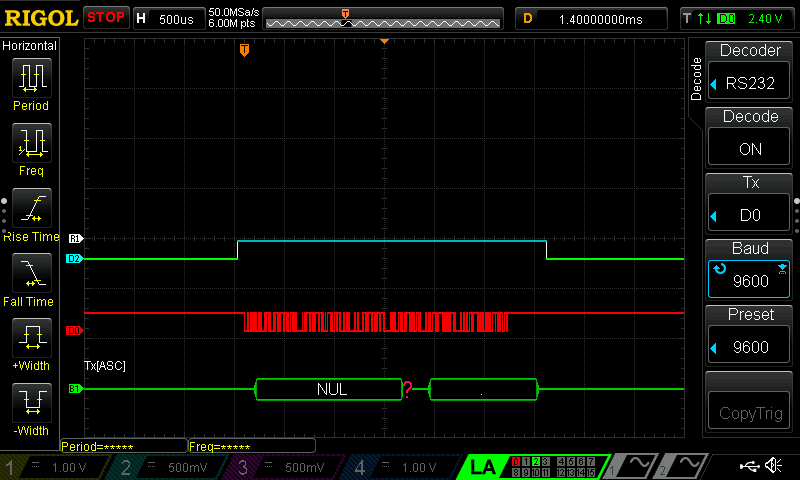
\includegraphics[scale=0.4]{figures/Scope_No_Delay115200.png}
    \caption{When 115200 baudrate is used, the \texttt{usleep()} function seems to sleep too long}
    \label{fig:scope_no_delay115200}
\end{figure}


\newpage

Things start to be really off when an extra byte delay is added in Listing \ref{lst:serial_write_delay} for the 115200 baudrate.
The data is still decent, but instead of an extra $\frac{1}{11520} * 1000000 = 86 \mu S$ that is added to the \texttt{DE} toggling, it seems that an additional $1900 \mu S$ have been added.
This can be seen in Figure \ref{fig:scope_extra_delay115200}.

\begin{figure}[H]
    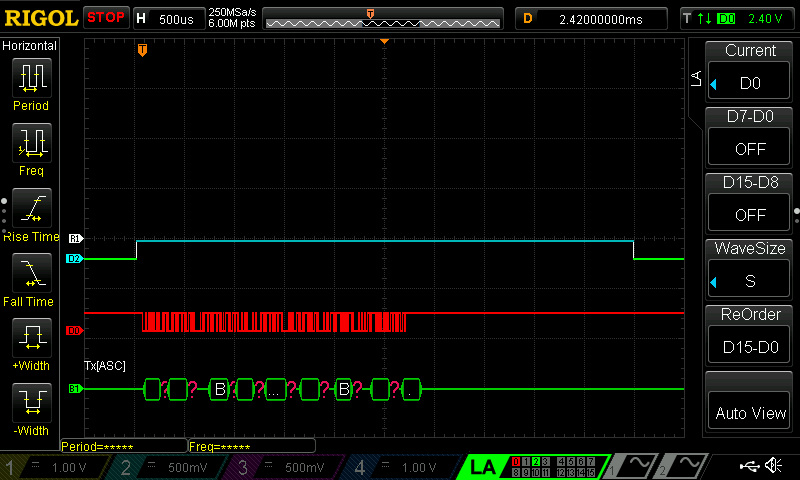
\includegraphics[scale=0.4]{figures/Scope_Extra_Delay115200.png}
    \caption{Things start to be really off when a 1 byte extra delay in Listing \ref{lst:serial_write_delay} is added on a baudrate of 115200}
    \label{fig:scope_extra_delay115200}
\end{figure}

This level of inaccuracy is very problematic because subsystems could potentially start sending their response when the \texttt{DE} pin is high for this long.
This code may actually work and be more accurate on a higher-performance processor such as on the Raspberry Pi 4 or change the Operating System to a  Real Time Operating System.
These are all hypothesis based on the observations made and the performance of the RPI Zero 2. \newline


\textbf{UPDATE:} This problem seems also to be an issue with a much faster CPU.
When sending with a baudrate of 115200 on the Raspberry Pi 4 there is also a delay after the last byte has been sent whilst this is not intentional.


\begin{figure}[H]
    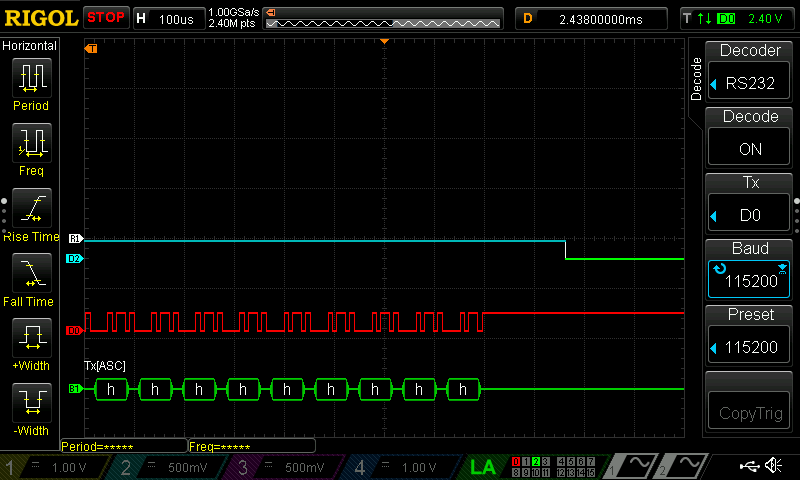
\includegraphics[scale=0.4]{figures/Scope_No_Delay115200_RPI4.png}
    \caption{Even on the Raspberry Pi 4 with a baudrate of 115200 and no extra delay, the \texttt{DE} toggle has a delay}
    \label{fig:scope_no_delay115200_rpi4}
\end{figure}

\newpage
\textbf{SOLUTION:} The old code was switching the \texttt{DE} pin on a software-level and was dependent on the \texttt{usleep()} function making the process unblocked and the Operating System actually scheduling the code as fast as possible to execute the next few lines after \texttt{usleep()} to toggle to \texttt{DE} pin.
In the new code we use \texttt{linux/serial.h} in order to have access to a \texttt{struct serial\_rs485} which we can configure to do the \texttt{DE} toggling in hardware/kernel level.
The example code from the Linux kernel in Listing \ref{lst:rs485_linux} was almost sufficient to get the job done


\begin{lstlisting}[frame=single, caption={Linux RS485 struct to define the \texttt{DE} toggling characteristics in hardware or in the kernel}, captionpos=b, label={lst:rs485_linux}, basicstyle=\small, style=CStyle]
#include <linux/serial.h>

/* Include definition for RS485 ioctls: TIOCGRS485 and TIOCSRS485 */
#include <sys/ioctl.h>

/* Open your specific device (e.g., /dev/mydevice): */
int fd = open ("/dev/mydevice", O_RDWR);
if (fd < 0) {
        /* Error handling. See errno. */
}

struct serial_rs485 rs485conf;

/* Enable RS485 mode: */
rs485conf.flags |= SER_RS485_ENABLED;

/* Set logical level for RTS pin equal to 1 when sending: */
rs485conf.flags |= SER_RS485_RTS_ON_SEND;
/* or, set logical level for RTS pin equal to 0 when sending: */
rs485conf.flags &= ~(SER_RS485_RTS_ON_SEND);

/* Set logical level for RTS pin equal to 1 after sending: */
rs485conf.flags |= SER_RS485_RTS_AFTER_SEND;
/* or, set logical level for RTS pin equal to 0 after sending: */
rs485conf.flags &= ~(SER_RS485_RTS_AFTER_SEND);

/* Set rts delay before send, if needed: */
rs485conf.delay_rts_before_send = ...;

/* Set rts delay after send, if needed: */
rs485conf.delay_rts_after_send = ...;

/* Set this flag if you want to receive data even while sending data */
rs485conf.flags |= SER_RS485_RX_DURING_TX;

if (ioctl (fd, TIOCSRS485, &rs485conf) < 0) {
        /* Error handling. See errno. */
}

/* Use read() and write() syscalls here... */

/* Close the device when finished: */
if (close (fd) < 0) {
        /* Error handling. See errno. */
}
\end{lstlisting}


Please keep in mind that for the Raspberry Pi, the reader has to do a few things such as setting GPIO 17 to an alternative function by loading the \texttt{miniuart-ctsrts.dbto} file from GitHub and in the \texttt{/boot/overlays} directory\footnote{\url{https://forums.raspberrypi.com/viewtopic.php?f=44\&t=241623\#p1473905}}.
The reader has to change the \texttt{/boot.config.txt} file as well (See Subsection \ref{subsec:rpitogglefix}). \newline

As of now there is no extra delay before- or after the message. This is because only delays expressed in milliseconds can be given with the Linux kernel RS485 module and a baudrate of 115200 is quite fast. The least amount of delay, which is 1 millisecond, is quite some time already when one sends on a 115200 baudrate.
Hence why it has been decided that as of now there is no need for an extra delay and we could always add a delay later if data turns out to be transmitted unreliable.

\newpage

\subsection{Raspberry Pi RS485 driver does not toggle \texttt{DE} pin - fix}
\label{subsec:rpitogglefix}

The Raspberry Pi has two UART modules and two different drivers. The main UART module is used to communicate to the on-board Bluetooth module and uses the PL011 driver. The other UART module uses the different miniuart driver and is less stable.
Recently the PL011 driver got updated and has support for hardware control (CTS/RTS) as well which is used by the Linux RS485 driver to toggle the Driver Enable (DE) pin.
However, when we disable Bluetooth by adding the \texttt{dtoverlay=disable-bt} in \texttt{/boot/config.txt} then UART0 should be available to us with the PL011 driver.
However, when one tries to configure the RS-485 driver with the code from Listing \ref{lst:rs485_linux} then we get the output that can be seen in Listing \ref{lst:rpi_error1}.

\begin{lstlisting}[caption={Output when one tries to communicate to \texttt{/dev/ttyAMA0} and Bluetooth is disabled}, captionpos=b, label={lst:rpi_error1}, basicstyle=\small, style=dos]
$ gcc test.c serial.c -o test
$ sudo ./test
[SERIAL] Failed to initialize the RS-485 driver with error 25
\end{lstlisting}

\textbf{SOLUTION:} We were not able to get it working with the Bluetooth driver being disabled and using the PL011 driver on \texttt{/dev/ttyAMA0}. However, we got it partially and very unreliably working by keeping the Bluetooth driver enabled and downloading a compiled dtoverlay script from GitHub\footnote{\url{https://github.com/HiassofT/AtariSIO/tree/master/contrib/rpi}} and place the \texttt{miniuart-ctsrts.dtbo} file in the \texttt{/boot/overlays/} directory.
Once that is done, the reader has to modify the \texttt{/boot/config.txt} file and the bottom few lines should be added

\begin{lstlisting}[caption={If UART is not enabled then add the first line as well in \texttt{/boot/config.txt}}, captionpos=b, label={lst:rpi_fix1}, basicstyle=\small, style=dos]
enable_uart=1
dtoverlay=miniuart-ctsrts
\end{lstlisting}

Since the \texttt{DE} toggling will happen on GPIO17, this pin should be in alternate function 5. We thought it had to be in alternative function 3 but that did not happen to work and might be for the PLA011 driver.
One could verify the alternate function of GPIO 17 with the command below

\begin{lstlisting}[caption={If UART is not enabled then add the first line as well in \texttt{/boot/config.txt}}, captionpos=b, label={lst:rpi_fix1}, basicstyle=\small, style=dos]
$ sudo raspi-gpio get 17
GPIO 17: level=0 fsel=2 alt=5 func=RTS1
\end{lstlisting}

If this is all done then the \texttt{DE} pin used in the Serial library should be toggled by the Linux kernel and the hardware peripheral.
Because of the UART design on the Raspberry Pi it does not happen to work reliable and sometimes for some mysterious reason the \texttt{DE} pin is toggled and immediately toggled again resulting in a very small pulse which can be seen in Figure \ref{fig:RPi_Uart_Bug}


\begin{figure}[H]
    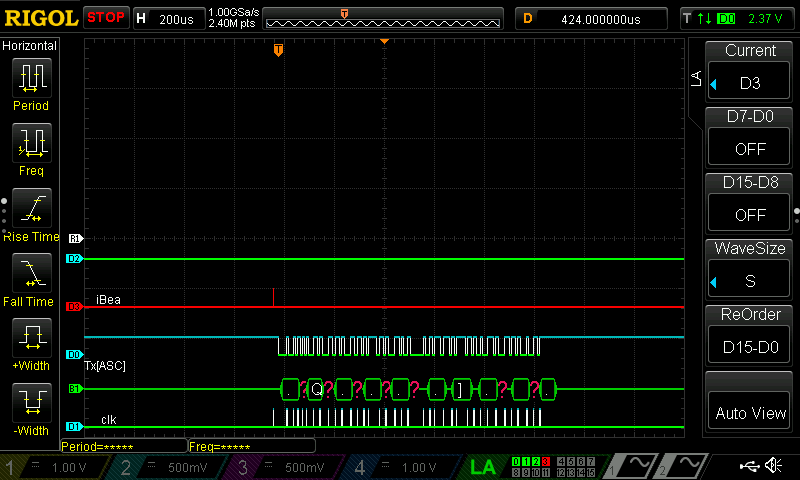
\includegraphics[scale=0.4]{figures/RPi_Uart_Bug.png}
    \caption{Hardware bug of the Raspberry Pi UART design}
    \label{fig:RPi_Uart_Bug}
\end{figure}

For this reason we strongly recommend to use the BeagleBone Black (BBB) as replacement platform for the OBC because it has true UART peripherals which aren't partially reserved for any other on-board device.
It does also run Linux and the Serial library should work more reliably.
